%%%%%%%% EIML@ICML 2026 WORKSHOP PAPER %%%%%%%%%%%%%%%%%
%
% Number sources: every number is read from results/analysis/SUMMARY.md or a JSON in
% results/analysis/ that it cites. Comments "% src: file:key" give the key next to each number.

\documentclass{article}

\usepackage{microtype}
\usepackage{graphicx}
\usepackage{booktabs}
\usepackage{flushend}
\usepackage{hyperref}

\newcommand{\theHalgorithm}{\arabic{algorithm}}

\usepackage[accepted]{eiml_icml2026}
\hypersetup{hypertexnames=false}
\makeatletter
\renewcommand{\ICML@appearing}{\textit{2nd Workshop on Epistemic Intelligence in Machine Learning (EIML@ICML 2026), Seoul, South Korea. Copyright 2026 by the author(s).}}
\makeatother

\usepackage{amsmath}
\usepackage{amssymb}
\usepackage{amsthm}

\theoremstyle{plain}
\newtheorem{theorem}{Theorem}[section]
\theoremstyle{remark}
\newtheorem{assumption}[theorem]{Assumption}

\icmltitlerunning{Where Cross-Question Structure in LLM Errors Comes From}

\begin{document}

\twocolumn[
\icmltitle{Where Cross-Question Structure in LLM Errors Comes From:\\
Shared Seeds, Shared Prompts, and Answer-Letter Preference}

\icmlsetsymbol{equal}{*}
\begin{icmlauthorlist}
\icmlauthor{Izhar Ali}{rowan}
\end{icmlauthorlist}
\icmlaffiliation{rowan}{Rowan University}
\icmlcorrespondingauthor{Izhar Ali}{aliizh94@rowan.edu}

\vskip 0.3in

\begin{abstract}
Disagreement among a language model's samples, or among the models of an
ensemble, is read as epistemic uncertainty: models that lack knowledge
should miss the same groups of questions. We ask when such structure
across the questions of a correctness matrix reflects shared knowledge
gaps, and when it comes from the evaluation pipeline or
from answer-letter preference; repeated samples of one model serve as
controls. We count eigenvalues of the question correlation
matrix above those produced by independent answers or, across models,
by a single ability per model. Within one model,
independent requests show no detectable direction, while a seed or
exemplar set shared across one round of samples creates directions. Across 24 greedily decoded models, the first direction
follows ability and the second is answer-letter preference: when the
options are rotated it follows the displayed letter, not the question,
and it rests mostly on one model. Counting a question correct only if it
is answered correctly in all four rotations leaves no excess at the
second eigenvalue, with low power against a second ability of typical
strength; a marginal excess at the third and fourth comes mostly from
two near-duplicate model pairs, partly from the letter-biased model. One letter-biased
model can thus pose as a second dimension of knowledge; options should be
rotated before an ensemble's error structure is read as epistemic.
\end{abstract}
]

\printAffiliationsAndNotice{}

%======================================================================
\section{Introduction}
\label{sec:intro}

Self-consistency samples a language model $K$ times on each question and
reads disagreement among the samples as uncertainty about the
answer~\citep{selfconsistency2023,selfcheckgpt2023,semanticentropy2024}.
Disagreement among the members of a deep
ensemble~\citep{lakshminarayanan2017} is read the same way, as epistemic
uncertainty, which comes from missing knowledge, rather than aleatoric
uncertainty, the noise that remains when the model is
known~\citep{kendall2017uncertainties,huellermeier2021aleatoric}.
A model that lacks some knowledge fails on the questions that need it,
and errors of different models are related: models often choose the same
wrong answer~\citep{correlatederrors2025}, and the scores of many models
are summarized by a few latent
factors~\citep{burnell2023structure,ruan2024observational,iqtest2025}.
We call the tendency of questions to be answered right or wrong together
\emph{cross-question structure}, and ask when it is evidence of shared
knowledge gaps and when it is an artifact of the pipeline (a shared seed,
shared exemplars) or of answer-letter preference.

The $k$th samples of all questions form \emph{pass}~$k$; like one ensemble member, a pass answers every question
once. Self-consistency samples each prompt by a separate request with its
own random numbers, so given the model, correctness on two questions of a
pass is independent by construction. A pipeline can still couple them:
one seed in a batched call's sampling parameters gives every prompt the
same random numbers, and the standard
5-shot MMLU prompt places one fixed set of exemplars before the questions
of a subject~\citep{mmlu2021}. Within one model, a test for such
structure is therefore a control: independent requests should show no structure, and a shared seed
or exemplar set should. Different models share no sampling noise, but
they differ in ability and in habits unrelated to knowledge: a model that
prefers one answer letter is right more often on the questions whose
correct option carries that
letter~\citep{zheng2024selectors,pezeshkpour2024order}.

We test a correctness matrix, passes or models by questions, for
eigenvalues of its question correlation matrix above what independent
answers produce~\citep{marchenkopastur1967,johnstone2001} or, across
models, one ability per model~\citep{rasch1960,lordnovick1968}. Each such
eigenvalue marks a shared \emph{direction}: a pattern of questions along
which the rows vary together.

\paragraph{Contribution and related work.} The tools are classical
(App.~\ref{app:background}), and spectral dimensionality measures
compared with a Marchenko--Pastur null, together with parallel analysis,
have been applied to item-level benchmark matrices, where binary spectra
are known to overstate
dimensionality~\citep{benchscope2026}. Letter preference and order
sensitivity are known for single
models~\citep{zheng2024selectors,pezeshkpour2024order}, as is the
influence of few-shot exemplars on the answer
distribution~\citep{zhao2021calibrate,min2022rethinking}.
\citet{ding2026agree} shows with an option-shuffle control that part of
a model's self-agreement is positional. In the option-level response
model of \citet{fei2026wrong}, a per-model positional preference barely
helps to predict held-out correctness (prediction accuracy 0.840 with it,
0.838 without); in a binary correctness matrix, which records no letter,
we find that removing one strongly biased model brings the second
eigenvalue down to within what one ability produces. Our contribution is not the method but
its controls and attribution: protocols that calibrate the test, an
option-rotation design, scored by the CircularEval rule
of~\citet{mmbench2024}, that attributes the second direction to letter
preference, and validity-checked one-ability nulls with measured power
and, for the main across-model test, size.
% src: Fei et al. 2026, Table 1 (5-fold held-out accuracy, full 0.8395 vs without delta 0.8382); attack2_citations.md

\begin{figure*}[t]
\centering
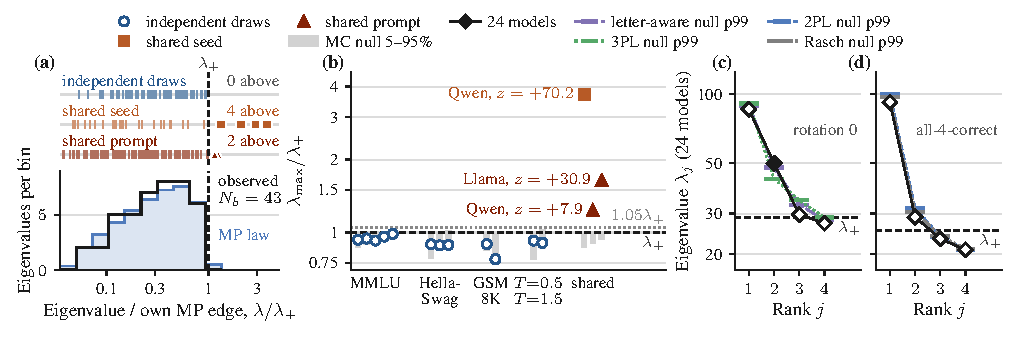
\includegraphics[width=\textwidth]{figures/fig_spectra.pdf}
\vskip -0.05in
\caption{\textbf{(a)}~Eigenvalues of $\mathbf{R}$ for three runs of
Qwen2.5-7B on MMLU ($K=100$): independent draws, shared seed and shared
prompt, divided by each matrix's own MP edge $\lambda_+$ (dashed);
markers: above the edge. Lower: histogram of the independent-draw run's
eigenvalues ($N_b=43$) and the MP law.
\textbf{(b)}~$\lambda_{\max}/\lambda_+$ for every within-model run
(Table~\ref{tab:runs}); grey bars: 5--95\% range of each run's Monte
Carlo null; dotted: $1.05\,\lambda_+$. \textbf{(c,d)}~The four largest
eigenvalues of the 24-model matrix (c)~in rotation 0 and
(d)~counting a question correct only if correct in all four
rotations, against the rank-matched 99th percentiles of two one-ability
nulls each: (c)~the letter-aware null and the 3PL; (d)~the 2PL and
Rasch. Only valid nulls are shown. Filled marker: above both nulls;
dashed: $\lambda_+$. The figure and the per-rank results of
Sec.~\ref{sec:across} use 1000 draws per null; the family-wise $p_T$
and percentiles of Sec.~\ref{sec:all4} on the full data, 2000 new draws;
App.~\ref{app:ensemble} gives the draw counts of all other results. In (d), $\lambda_4=20.83$ equals the
2PL rank-4 99th percentile (20.85) within Monte Carlo error.}
% src: draw counts: v3_B_leave_one_out.json:meta.n_draws_per_null 1000; v3_G_familywise.json:meta.n_draws.{G1 2000, G4 1000}; v3_I_llama.json:meta.n_draws.{I1 2000, I2 1000}; v3_H_followup.json:meta.n.H2_null_draws 1000

% src: v3_C_rotations_A.json:C3_rotation_invariant.all4_correct.spectrum.top_eigs[3] (20.83); suite.nulls.2pl_post.rank_eigs_p99[3] (20.85); MC p 0.012: SUMMARY.md C(3)
\label{fig:spectra}
\end{figure*}

%======================================================================
\section{A spectral test for cross-question structure}
\label{sec:method}

Entry $c_{ki}$ of the correctness matrix $\mathbf{C}$ is 1 when row $k$
answers question~$i$ correctly and 0 otherwise. Row $k$ is pass $k$ within one
model and model $m$ across models. A question that every row gets right,
or none does, carries no correlation, so we keep the questions that vary:
within a model, the $N_b$ \emph{borderline} questions with pass rate
$\varepsilon<f_i<1-\varepsilon$, $\varepsilon=0.05$; across models, the
\emph{split} questions, which some models answer correctly and others do
not. Let $\mathbf{R}$ be the Pearson correlation matrix of the kept
columns over the rows. If the questions are independent, the eigenvalues
of $\mathbf{R}$ spread around 1 and, as rows and columns grow with their
ratio $\gamma$ (kept columns over rows) fixed, follow the
Marchenko--Pastur (MP) law, whose upper edge is
$\lambda_+=(1+\sqrt\gamma)^2$~\citep{marchenkopastur1967}. An
eigenvector gives the question loadings of its direction; a row's
\emph{score} on it is the projection of its standardized row.

\paragraph{Within one model.} For Gaussian data, the largest eigenvalue
$\lambda_{\max}$ fluctuates near $\lambda_+$ on the Tracy--Widom scale
$\sigma_{\mathrm{TW}}$, the size of its typical
fluctuation~\citep{johnstone2001}, and
$z=(\lambda_{\max}-\lambda_+)/\sigma_{\mathrm{TW}}$ measures its distance
above the edge. Because no theorem we know gives this limit for
sample-centered binary entries (App.~\ref{app:background}), we compare each $z$ with a Monte Carlo null
of 1000 matrices of independent Bernoulli entries at the observed pass
rates, with the filter re-applied (App.~\ref{app:stats}). The MP count is
the number of eigenvalues above $\lambda_+$; the buffered count, above
$1.05\,\lambda_+$, leaves a margin for the fluctuation of $\lambda_{\max}$
and is positive in 0.65\% and 0.35\% of simulations without shared
structure at the pass rates of Qwen2.5-7B and Llama-3-8B on MMLU
(App.~\ref{app:power}).
% src: item03_power.json:models.<MMLU Qwen2.5-7B T1.0|MMLU Meta-Llama-3-8B>.scenarios[0].power_mp_buffered_1p05 (0.0065, 0.0035)

\paragraph{Across models.} Here $\lambda_+$ is not the reference: a
one-ability model with a logistic response can produce a
second eigenvalue above $\lambda_+$ by itself (Sec.~\ref{sec:all4}).
We therefore compare each eigenvalue $\lambda_j$ with the $j$th
eigenvalue of 1000 matrices simulated from a one-ability model fitted to
the data. In the two-parameter logistic (2PL)
model~\citep{lordnovick1968}, model $m$ answers question $i$ correctly
with probability $\sigma(a_i(\theta_m-b_i))$, with one ability $\theta_m$
per model and a difficulty $b_i$ and slope $a_i$ per question; Rasch sets
every slope equal~\citep{rasch1960}, and the 3PL adds a guessing floor of
0.25. In the \emph{letter-aware} null, a model knows the answer with the
2PL probability and otherwise guesses letter $L$ with its own probability
$\pi_m(L)$; the \emph{uniform know-or-guess} null guesses uniformly. A
null rejects rank $j$ when $\lambda_j$ exceeds the 99th percentile of its
$j$th eigenvalue; ranks $2,3,\ldots$ rejected in a row are
\emph{directions beyond ability}. A null counts as evidence only if it is
\emph{valid}, that is, it reproduces the ability eigenvalue: the
observed $\lambda_1$ lies between its 1st and 99th percentiles. An excess can also spread over
several ranks. The \emph{family-wise test} therefore takes the largest
percentile of the observed $\lambda_2$, $\lambda_3$ and $\lambda_4$
among the null draws, and compares it with the same maximum in each of
2000 new null draws, giving its $p$-value $p_T$
(App.~\ref{app:ensemble}). We fixed this statistic, its ranks, the
sibling groups of Sec.~\ref{sec:all4} and the validity rule before the
test's run, after an audit of an earlier draft of this analysis had
computed a similar statistic on the same data. The first analyses used
an earlier validity convention; the pair and single-model follow-ups
are post hoc.
% src: v3_G_familywise.json:meta.n_draws.G1 (2000)

\paragraph{Runs.} Within one model (App.~\ref{app:data}), the
\emph{independent} protocol gives every (question, pass) pair its own
seed, as self-consistency does; in the \emph{shared-seed} protocol all
questions of a pass use one seed; in the \emph{shared-prompt} protocol
each pass places its own five MMLU development questions, with their
answer letters, as exemplars before every question. Twelve
independent-draw runs cover five instruction-tuned models on
MMLU~\citep{mmlu2021} and three on
HellaSwag~\citep{zellers2019hellaswag} at temperature 1, and Qwen2.5-7B on
GSM8K~\citep{gsm8k2021} at two output lengths and on MMLU at
temperatures 0.5 and 1.5 (Table~\ref{tab:runs}); three \emph{shared-component} runs, one
shared-seed and two shared-prompt, use MMLU with $K=100$. Across models, 24 models (23
instruction-tuned, one base) of 0.5B to 22B parameters from ten
families
answer the 500 MMLU questions by greedy decoding, in four
\emph{rotations}: rotation $r$ shows original option $j$ at letter
position $(j+r)\bmod 4$; rotation 0 is the original.
% src: item01_within_table.json:runs[*].{K, temperature, N} (MMLU K 100; HellaSwag K 50; GSM8K 256/1024 and MMLU T0.5/T1.5 K 30)
% src: item01_within_table.json:runs[0..9].temperature (1.0), runs[10,11].temperature (0.5, 1.5); GSM8K 256/1024 tokens: Table tab:runs

%======================================================================
\section{Results}
\label{sec:results}

\subsection{Controls within one model}
\label{sec:iid}

In all 12 independent-draw runs the largest eigenvalue lies below the MP
edge (Fig.~\ref{fig:spectra}a,b), and every $z$ lies between the 10th and
the 84th percentile of its Monte Carlo null; the counts stay zero at six
borderline thresholds (App.~\ref{app:stats}). The test finds no hidden
coupling in our pipeline, within its power: in simulations where each
answer is decided by a normal variable and these variables correlate at
$\rho$ across a pass's borderline questions (App.~\ref{app:power}), at
$\rho=0.05$ the MP count detects the coupling in every matrix at
Llama-3-8B's $N_b=173$ and in 47\% at Qwen2.5-7B's $N_b=43$, and a
nine-question cluster at $\rho=0.2$ in at most 23\%.
% src: item01_within_table.json:runs[*].mc_null_z.percentile_of_obs (min 0.102, max 0.835); runs[*].eps_sweep[*].mp_count (all 0)
% src: item03_power.json:models.<MMLU Meta-Llama-3-8B>.scenarios[3].power_mp_strict (1.0); <MMLU Qwen2.5-7B T1.0>.scenarios[3].power_mp_strict (0.47); scenarios[7].power_mp_strict (0.232)

In the shared-component runs, $z$ exceeds every draw of its null
and two to four eigenvalues exceed $1.05\,\lambda_+$; the
directions follow the shared input (App.~\ref{app:mechanism}). A shared
seed gives one answer letter the same random boost in every question of
a pass, so gold letter explains 73\% of the variance of the top
eigenvector's loadings ($\eta^2=0.73$, permutation $p=0.0002$). Llama-3-8B copies the shared
exemplars' answer letters ($\eta^2=0.53$, $p=0.0002$). Qwen2.5-7B's
shared-prompt direction does not group by gold letter ($p=0.094$), but
two passes whose exemplars share a question answer more alike than other pairs ($p=0.0005$).
% src: item02_shared_randomness.json:runs.<run>.mc_null_z.percentile_of_obs (1.0 each); runs.<run>.mp_count_buffered (4, 2, 2)
% src: item02_shared_randomness.json:runs.<sharedseed Qwen>.top_pc.loadings_eta_sq_by_gold_letter.{eta_sq 0.73, perm_p 0.0002, n_perm 5000}; <sharedprompt Llama> (0.53, 0.0002); <sharedprompt Qwen> perm_p (0.094)
% src: item02_shared_randomness.json:runs.<sharedprompt Qwen>.exemplar_alignment.pass_pair_similarity_shared_exemplars_borderline.{z_vs_null 10.7, perm_p_upper 0.0005}

\subsection{Across models: a second direction, from letter preference}
\label{sec:across}

In rotation 0 the four largest eigenvalues of the 24-model matrix (460
split questions) are 85.9, 49.9, 29.7 and 27.3, against
$\lambda_+=28.92$. The models' scores on eigenvector 1 correlate with
accuracy at $r=0.94$: it is the ability direction. Four nulls are valid:
the letter-aware, 3PL and uniform know-or-guess nulls
($\lambda_1$ at their 86.7th, 76.4th and 98.7th percentiles) and the
soft-preference null (below);
the 2PL and Rasch put $\lambda_1$ above all their draws. Each of the
first three rejects rank 2 and no other (Fig.~\ref{fig:spectra}c), and the family-wise test rejects all three ($p_T=0.002$).
% src: v3_B_extra.json:suite.observed.top_eigs; item07_across_model.json:observed.{n_split 460, lambda_plus 28.92}; v3_B_extra.json:letter_analysis.eigenvectors[0].model_score_corr.accuracy.r (0.94)
% src: v3_F_softpref.json:step1_construction_family.table.full.rot0.{observed_pct_rank1to4_by_null.{letter_post 86.7, 3pl_post 76.4, kg_uniform4 98.7, 2pl_post 100, rasch_jml 100}, ranks_above_p99_by_null.{letter_post,3pl_post,kg_uniform4} ([2])}
% src: v3_G_familywise.json:G1_familywise.by_score_and_null.rot0.{3pl_post,letter_post,kg_uniform4}.{valid true, p_T 0.0020 (=4/2001)}

Eigenvector 2 is answer-letter preference. Its question loadings group
by gold letter ($\eta^2=0.48$, $p=0.0002$), and the models' scores on it
correlate with their fraction of answers that are D at $r=-0.90$
(Fig.~\ref{fig:letters}a) and with their fraction that are A at
$r=0.76$. Within one rotation a question's gold letter
is tied to its content, so this grouping cannot separate the two;
rotating the options can. In rotations 1--3 we correlate each
question's loading on eigenvector 2 (matched by the models'
scores) with its own rotation-0 loading and with the rotation-0 mean
loading of questions whose gold letter is its new one. A direction of
question content would follow the own loading; this one follows the
shown letter ($r=0.60$ to 0.64, against $-0.06$ to 0.16;
Fig.~\ref{fig:letters}b).
% src: v3_B_extra.json:letter_analysis.eigenvectors[1].{eta_sq_by_shown_gold_letter.{eta_sq 0.482, perm_p 0.0002}, model_score_corr.share_D.r -0.90, model_score_corr.share_A.r 0.764}
% src: v3_C1b_letter_following.json:A.eigvec2.{1,2,3}.{r_shown 0.64/0.60/0.61, r_direct -0.06/0.16/-0.003, model_score_match_abs_r 0.98/0.96/0.95}

The direction rests mostly on one model, Llama-3.2-1B, whose estimated
letter preference when it guesses puts probability 0.90 on A. Removing it lowers
$\lambda_2$ from 49.9 to 35.0, below the 99th percentiles of the 3PL and
letter-aware nulls refitted to the other 23 models (40.1 and 38.1), so
the per-rank rule finds no direction beyond ability; removing any other
single model leaves $\lambda_2$ between 47.1 and 52.4. A post hoc
family-wise test still rejects both nulls ($p_T=0.0035$ and 0.015): a
weaker excess remains at ranks 3--4, where the letter grouping moves
(eigenvector 3, $\eta^2=0.21$).
% src: v3_C_rotations_A.json:kg_fits_4_rotations.letter_preference.<meta-llama/Llama-3.2-1B-Instruct>.pi_A_B_C_D[0] (0.90)
% src: v3_B_leave_one_out.json:leave_one_out_spectra.<meta-llama/Llama-3.2-1B-Instruct>.{rot0.top_eigs[1] (35.0), rot0_eta_sq_gold_letter_eigvec_1to4[2] (0.214)}; v3_summary_derived.json:loo_rot0_lambda2_min_max_without_llama_3_2_1b_removal ([47.1, 52.4])
% src: v3_B_leave_one_out.json:without_llama_3_2_1b.rot0_suite.nulls.{3pl_post.rank_eigs_p99[1] 40.07, letter_post.rank_eigs_p99[1] 38.07}; v3_F_softpref.json:step1_construction_family.table.no_llama1b.rot0.ranks_beyond_ability_valid_nulls ({3pl_post 0, letter_post 0})
% src: v3_I_llama.json:I1_without_llama1b.table.rot0.{3pl_post.{valid true, p_T 0.0035, pct_rank1to4 [96.6, 48.2, 98.5, 99.9]}, letter_post.{valid true, p_T 0.0150, pct_rank1to4 [88.55, 72.2, 99.2, 99.5]}} (post hoc, prereg_I.md)

The letter-aware null lets the preference act only on guesses and
under-reproduces $\lambda_2$. In a \emph{soft-preference} (SP) model
the preference also tilts choices a model partly knows, and ability is
the only link between questions; the letter-aware null rejects rank 2
in 60\% of datasets simulated from it. The SP null is also valid
($\lambda_1$ at its 85.7th percentile); it rejects rank 2 (calibrated
$p=0.010$) but not family-wise ($p_T=0.079$), and its fit fails a
predictive check (App.~\ref{app:ensemble}). Neither model thus
reproduces all of $\lambda_2$, but the rotation test leaves little room
for a part that follows question content: we read the remainder as
letter preference that neither model captures fully, not excluding a
small content part.
% src: v3_F_softpref.json:step2b_step1_nulls_under_soft_preference_truth.summary.rot0.letter_post.frac_rank2_above_p99 (0.595)
% src: v3_G_familywise.json:G5_single_validity_rule.sp_table_A2.full.rot0.{plain_valid true, lambda1_pct 85.7, rank2_cal_p 0.010, rank2_cal_p_mc 0.0149}; G1_familywise.by_score_and_null.rot0.sp_common_tau.p_T (0.07946 -> 0.079)

\subsection{All-4-correct scoring: a marginal excess, mostly from two model pairs}
\label{sec:all4}

To remove letter preference, we count a question correct for a model
only when the model answers it correctly in all four rotations, the
CircularEval rule~\citep{mmbench2024}. The gold option appears once at
each letter over the rotations, so a model that only guesses by letter is
correct in all four with probability $\prod_L\pi_m(L)\le1/256$, the same
for every question. In this \emph{all-4-correct} matrix (391 split
columns, $\lambda_+=25.36$) the eigenvalues are 92.1, 29.0, 23.3 and 20.8
(Fig.~\ref{fig:spectra}d). The valid nulls are the 2PL and Rasch
($\lambda_1$ at their 31.5th and 54.2nd percentiles); the other nulls
miss $\lambda_1$. The 99th percentile of $\lambda_2$ is 31.9
under the 2PL and 30.2 under Rasch, above $\lambda_+$, so one ability
alone can lift a second eigenvalue above the edge; the observed
$\lambda_2$ lies below both: no second direction separates at rank 2.
% src: v3_C_rotations_A.json:C3_rotation_invariant.all4_correct.spectrum.{n_cols 391, lambda_plus 25.36, top_eigs}
% src: v3_G_familywise.json:G1_familywise.by_score_and_null.ge4.{2pl_post.{valid true, pct_rank1to4[0] 31.45, rank_eigs_p99[1] 31.94}, rasch_jml.{valid true, pct_rank1to4[0] 54.15, rank_eigs_p99[1] 30.18}, {3pl_post,ba_a4,kg_letter4,kg_uniform4,fixed_margin,sp_common_tau}.valid false}

The excess lies lower: $\lambda_3$ and $\lambda_4$ sit at the 98.5th and
99.1st percentiles of the 2PL and the 97.0th and 98.6th of Rasch, and the
family-wise test rejects both nulls ($p_T=0.026$ and 0.041). Under
one-ability truth the test rejects in up to 8.7\% of datasets at the 5\%
level; calibrated against them, the observed $p_T$ are 0.017 to
0.057, a marginal excess (App.~\ref{app:ensemble}).
% src: v3_G_familywise.json:G1_familywise.by_score_and_null.ge4.{2pl_post.pct_rank1to4 [31.45, 71.8, 98.45, 99.1], rasch_jml.pct_rank1to4 [54.15, 94.55, 96.95, 98.6], 2pl_post.p_T 0.0265, rasch_jml.p_T 0.0415}
% src: v3_H_followup.json:H1_size_under_one_ability_truth.by_truth_and_null.<truth>.<null>.{fp_valid_and_p_T_lt_alpha (max: rasch truth / 2pl null 0.087), calibrated_p_of_real (0.033, 0.047, 0.057, 0.017)}

It comes mostly from two near-duplicate model pairs. Keeping one model
of each of four sibling groups (versions or fine-tunes of one base model
at one size), in all 24 combinations, removes the rejection, while
removing as many other models at random does not
(App.~\ref{app:ensemble}). A post hoc follow-up narrows this to two
pairs: removing one model each of Phi-3-mini/Phi-3.5-mini and
Meta-Llama-3-8B/Llama-3.1-8B gives $p_T$ 0.22 to 0.69 (2PL) and 0.32 to
0.38 (Rasch), above all 190 removals of two other models (at most 0.099
and 0.133). Removing the near-duplicates Mistral-7B v0.2 and v0.3 keeps
the rejection ($p_T=0.019$ under both). The pair excess may reflect
knowledge gaps shared through common training data, or another shared
artifact such as contamination; we did not test which. Without Llama-3.2-1B
alone the family-wise test no longer rejects ($p_T$ 0.06 and 0.089), so part of the
excess depends on that model. No factor shared across the ensemble is
detected, at low power.
% src: v3_H_followup.json:H3_baselines.{n_models_max_share_gt_0p5 3, letter_shares_rotation0, residual_corr.{n_pairs 276, sibling_pairs[0].rank 1, sibling_pairs[1].rank 2}}
% src: v3_G_familywise.json:G4_siblings.sibling.ge4.{2pl_post.p_T_min_median_max [0.087, ., 0.654], rasch_jml [0.124, ., 0.691], n_reject_raw_either_null 0}; G4_siblings.random_control.ge4.{n_reject_raw_both_nulls 24, 2pl_post max 0.047, rasch_jml max 0.046}
% src: v3_H_followup.json:H2_pair_removal_vs_reference.by_null.{2pl_post,rasch_jml}.{pair_removals[*].p_T (0.219-0.685; 0.322-0.382), reference_n 190, reference_max (0.0989, 0.1329)}; raw_v3_H_h2.json:subsets[116] (Mistral-7B v0.2 + v0.3: 2pl_post.p_T 0.019, rasch_jml.p_T 0.019)
% src: v3_I_llama.json:I1_without_llama1b.table.ge4.{2pl_post.{valid true, p_T 0.0595}, rasch_jml.{valid true, p_T 0.0890}} (post hoc, prereg_I.md)

Three limits qualify this result (App.~\ref{app:ensemble}). First,
all-4-correct removes a preference only if it acts when a model guesses;
the SP null, which lets it act on every choice, is not valid on
all-4-correct. Second, scores that do
not bound guessing give no reliable verdict: on ``correct in at least
two (or three) of four'', the 2PL test rejects one ability, but also in
98.5\% (58\%, indicative only, from an invalid fit) of datasets simulated from the
SP fit, which has no second factor; not every valid null rejects. We chose all-4-correct for its guessing bound, not for
its verdict. Third, power is low: a second ability planted on the 180
STEM questions with about a typical fitted slope is detected in 6\%
(2PL) and 8\% (Rasch) of datasets by the per-rank rule and in 34 and
21\% by the family-wise test (indicative rates: invalid SP fit).
% src: v3_G_familywise.json:G5_single_validity_rule.sp_table_A2.full.{ge4,ge3}.{plain_valid false, lambda1_pct 0.0}; ge2.plain_valid true
% src: v3_G_familywise.json:G2_calibration_under_SP_truth.{ge2.2pl_post.fp_valid_and_p_T_lt_alpha 0.985, ge3.2pl_post.fp_valid_and_p_T_lt_alpha 0.575}; G1_familywise.by_score_and_null.{ge2,ge3}.* (valid nulls that reject: see App.)
% src: raw_v3_F_sp_fits.npz:full__tau__sigma4__a (median |a| 1.076); v3_F_power.json:meta.block (180 STEM); v3_G_familywise.json:meta.n_draws.G3_datasets_per_s (200)
% src: v3_G_familywise.json:G3_power.{1,2}.{2pl_post,rasch_jml}.{detect_G1_raw (0.335, 0.205; 0.92, 0.87), per_rank_rule_rank2_above_p99_and_valid (0.055, 0.075; 0.805, 0.795)}

%======================================================================
\section{What is not shown}
\label{sec:limits}

Letter preference and the two pairs are the largest structure beyond
ability we find, not necessarily the only one. We test
correctness only, not log-probabilities, answer distributions, semantic
clusters or reasoning traces. The test cannot exclude small clusters of
questions within a model, nor a weaker second factor across models
(Sec.~\ref{sec:all4}); power for structure carried by a few models was
not simulated. Architecture, family, scale, data, instruction tuning and
decoding vary together in the ensemble; one architecture trained with
several seeds, or a dropout mask shared by a
pass~\citep{mcdropout2016}, would isolate a training seed or a shared
parameter perturbation. The within-model runs cover only instruction-tuned
models of 1.7B to 8B parameters, and the ensemble 500 MMLU questions.
Per-rank thresholds
are uncorrected over the nulls and scores of Table~\ref{tab:family}.

%======================================================================
\section{Discussion}
\label{sec:discussion}

One strongly letter-biased model can pose as a second dimension of
knowledge in a correctness matrix. Item-level factor and item response
analyses~\citep{metabench2025,benchscope2026,jeirt2025} and agreement on
the same wrong answer~\citep{correlatederrors2025} may contain the same
confound; we have not tested them. Before reading an ensemble's errors as epistemic, as in cross-model
uncertainty scores~\citep{hamidieh2025}, one should
rotate the options (four answers per question), score a question correct
only in all rotations, and test the remaining spectrum family-wise
against valid one-ability nulls, with near-duplicates in mind.

{\footnotesize
\bibliography{references}
\bibliographystyle{icml2026}
}

%======================================================================
\appendix
\renewcommand{\thefigure}{A\arabic{figure}}
\renewcommand{\thetable}{A\arabic{table}}
\renewcommand{\theHfigure}{A\arabic{figure}}
\renewcommand{\theHtable}{A\arabic{table}}
\setcounter{figure}{0}
\setcounter{table}{0}

%======================================================================
\section{Background}
\label{app:background}

This appendix describes the sampling-based uncertainty methods whose
samples' correctness the paper tests, and states the classical results
behind the tests: random-matrix limits for independent variables and item
response models.

\paragraph{Sampling-based uncertainty.} Sampling-based methods for
language
models~\citep{selfconsistency2023,selfcheckgpt2023,semanticentropy2024}
estimate uncertainty from the spread of one model's samples, and
\citet{mctemp2025} study how the sampling temperature affects these
estimates; a model can also be asked to evaluate whether its own answers
are true~\citep{kadavath2022}. In a correctness matrix, the spread of one
model's samples on question~$i$ is the Bernoulli variance $p_i(1-p_i)$,
set by that question alone. The paper asks whether this spread also has
the structure of an ensemble's disagreement, in which members are right
or wrong on groups of questions together.
\citet{illusionofstochasticity2026} show that language models do not
reliably sample from a target distribution when asked to, a different
property of sampled output from the one tested here.

\paragraph{Random-matrix tests for the number of factors.} A factor
shared by many variables lifts an eigenvalue of their sample correlation
matrix beyond the Marchenko--Pastur edge $\lambda_+$ of
Section~\ref{sec:method}: $n$ variables with pairwise correlation
$\kappa$ have a population eigenvalue of $1+(n-1)\kappa$. This eigenvalue
grows with $n$, so an eigenvalue test can detect a correlation smaller
than the sampling noise of one pairwise correlation, about $1/\sqrt{K}$.
Comparing sample eigenvalues with the MP edge is how
\citet{laloux1999} and \citet{plerou1999} separate market factors from
noise in stock-return correlations. The MP law holds for the sample
covariance matrices of independent entries with finite
variance~\citep{marchenkopastur1967,baisilverstein2010} and, for
i.i.d.\ entries, for their sample correlation
matrices~\citep{jiang2004correlation}.
\citet{johnstone2001} showed for Gaussian data that the largest
eigenvalue, minus the edge and divided by
$\sigma_{\mathrm{TW}}=(1+\sqrt\gamma)(1+1/\sqrt\gamma)^{1/3}K^{-2/3}$,
converges to the Tracy--Widom distribution. For sample correlation
matrices, \citet{baopanzhou2012} proved this limit for entries with a
symmetric distribution and no centering, with fewer variables than
observations, and with centering only for Gaussian entries;
\citet{pillaiyin2012} removed the symmetry condition and allowed more
variables than observations, still without centering. Our $\mathbf{R}$ is
centered at the sample means of Bernoulli columns with unequal pass
rates; no theorem we know covers sample-mean centering of non-Gaussian
entries, so the Monte Carlo null, not the limit, calibrates $z$.

\paragraph{Item response models.} Item response models come from
educational testing, where each test-taker has an ability and each
question a difficulty; here the test-takers are language models. In the
Rasch model~\citep{rasch1960} model $m$ answers question $i$ correctly
with probability $\sigma(\theta_m-b_i)$, with $\sigma$ the logistic
function: the probability rises with ability $\theta_m$, falls with
difficulty $b_i$, and is $1/2$ when the two are equal. The 2PL
model~\citep{lordnovick1968} adds a slope $a_i$, giving
$\sigma(a_i(\theta_m-b_i))$; a larger slope makes the probability rise
more sharply with ability. The 3PL form adds a guessing floor, here
$0.25+0.75\,\sigma(a_i(\theta_m-b_i))$ for four options. All are
one-factor models: ability is the only source of dependence between
questions. Such a model can still place more than one eigenvalue of a
24-row correlation matrix above $\lambda_+$ (Section~\ref{sec:method}),
and the all-4-correct eigenvector 2 follows question difficulty
(App.~\ref{app:ensemble}).

%======================================================================
\section{Data collection}
\label{app:data}

Every matrix in the paper comes from the protocol below; the last
paragraphs check the scoring of unparseable replies and the truncation on
GSM8K, and record how the data were collected.

\paragraph{Questions.} MMLU: 500 test questions, ten drawn at random from
each of the first 50 subjects in alphabetical order. HellaSwag: 200
validation items, a random sample stratified by activity label. GSM8K:
the first 100 test problems. Each question is matched to its exact
dataset row. The shared-prompt exemplars come from the 285 MMLU
development questions: pass $k$ uses five drawn at random from all
subjects, independently of the other passes, so two passes can share an
exemplar. The set is the same for every question of the pass and in
both shared-prompt runs.

\paragraph{Prompts and decoding.} Every model receives one user message
rendered with its own chat template; Phi-2, which has none, receives the
raw text. Prompts are tokenized with each model's own tokenizer and
checked against an independent reference tokenization. In the
shared-prompt protocol, the five exemplars, each followed by its answer
letter, sit in this message between the instruction and the question.
Generation uses vLLM 0.23.0 in bfloat16 with temperature $T$,
top-$p=1$, top-$k$ disabled, min-$p=0$, repetition penalty 1.0, no
presence or frequency penalty, and at most 8 new tokens for MMLU and
HellaSwag and 256 (or 1024) for GSM8K. Greedy decoding is $T=0$. In the
independent and shared-prompt protocols, every sample $(k,i)$ has its
own seed, distinct from every other seed of the run; in the shared-seed
protocol, all questions of pass $k$ share one seed, and the seed changes
from pass to pass. vLLM gives each seeded request its own random-number
generator, so a request's sampling noise depends on its seed, not on its
position in a batch, and requests with different seeds do not share
noise (App.~\ref{app:mechanism}).

\paragraph{Rotations and replicates.} The 24 models answer every
question in all four rotations, with deterministic kernel settings. GPU
kernels can still differ between engine starts, so the ensemble was
collected twice, with separate engine starts (replicates A and B). The
paper reports replicate A.

\paragraph{Scoring.} A multiple-choice reply is read as letter X when it
begins with X, after optional ``Answer:'', parenthesis or bold markers,
followed by punctuation, a line end, or words that do not negate or
hedge the letter; or when its first line says ``the answer is X'' or a
similar phrase. A reply that names several letters, negates its letter,
or cannot be read this way is unparseable and scored wrong. The rule is
fixed by unit and property-based tests. The GSM8K prompt asks for the
final answer after ``\#\#\#\#''; a reply is correct when the number after
its last ``\#\#\#\#'', or else its last number, equals the gold answer.

\paragraph{Unparseable replies.} In the sampled runs at most 1.65\% of
replies are unparseable (Llama-3-8B on HellaSwag), and the shared-seed
run and Qwen2.5-7B's shared-prompt run have none. In the ensemble,
Mistral-7B v0.2 has 12.4\% and every other model at most 9.6\%. We either
drop every question with an unparseable reply or replace each
unparseable reply by the mean correctness of the question's parseable
replies. Either way, every count of the independent-draw runs stays at
zero, and the MP and buffered counts of Llama-3-8B with a shared prompt
stay at two. Across models, we rerun the valid nulls on both variants
(Table~\ref{tab:fw}). On all-4-correct, the family-wise rejection
survives imputation and dropping the 95 questions whose all-4-correct
score depends on an unparseable reply, but not dropping all 217
questions with any unparseable reply, which keeps 236 of 391 columns and
has less power. In rotation 0, imputation leaves rank 2 above the
letter-aware and 3PL 99th percentiles; dropping the 112 affected
questions moves it to the 98.3rd percentile of the letter-aware null,
while the 3PL still rejects it and the family-wise test rejects under
both ($p=0.013$ and 0.004).
% src: item13_unparseable.json:rates_sampled_runs.<hellaswag Llama>.unparseable_rate (0.0165); rates_greedy_24.<Mistral-7B-v0.2>.unparseable_rate (0.124); <zephyr-7b-beta> (0.096, the next largest)
% src: item13_unparseable.json:within_model_sensitivity.*.{drop_questions_with_any_unparseable,impute_question_mean}.mp_count_* (0 for iid; 2/2 for Llama shared prompt)
% src: v3_G_familywise.json:G6_unparsed_variants.{ge4__drop_affected.n_questions_dropped 95, ge4__drop_any.{n_questions_dropped 217, n_cols 236}, rot0__drop.{n_questions_dropped 112, nulls.letter_post.pct_rank1to4[1] 98.3, nulls.{letter_post,3pl_post}.p_T (0.013, 0.004), nulls.3pl_post.ranks_beyond_ability 1}, rot0__impute.nulls.*.ranks_beyond_ability (1, 1)}

\paragraph{Truncation on GSM8K.} At 256 new tokens, 55\% of
Qwen2.5-7B's chain-of-thought replies reach the limit. Most of them stop
before the final answer, and the scorer then reads the last number of an
unfinished calculation: 13.6\% of truncated replies are correct, against
96.7\% of complete ones. Accuracy is 51.0\% at 256 tokens and 90.3\% at
1024 tokens. The run still tests independence: truncation changes which
answers are correct, not whether two questions of a pass share a cause.
% src: item12_temperature_gsm8k.json:gsm8k.256.{share_length_truncated 0.550, accuracy_truncated 0.136, accuracy_complete 0.967, accuracy 0.510}; gsm8k.1024.accuracy (0.903)

\paragraph{Collection history.} The data were collected anew after two
rounds of checks. The first found a scorer that accepted a reply
beginning with the gold letter as a word (``Based on \ldots'' as B) and a
question loader that matched questions by a text prefix shared by some
MMLU questions; the second found that three tokenizers (DeepSeek-LLM-7B,
Yi-1.5-6B, OLMo-2-7B) were loaded incorrectly, which changed those
models' prompts in the ensemble. Each defect was fixed and covered by a
test. The sampled runs were collected once with the fixed loader and
scorer and re-scored with the final parser; the ensemble was collected
again for all 24 models, in four rotations and two replicates.

%======================================================================
\section{Test statistics and checks}
\label{app:stats}

This appendix lists the within-model runs, states the independence that
the within-model test assumes and what it implies for the spectrum,
defines the Horn count, checks the independence on the data, and varies
the borderline threshold.

\begin{table}[t]
\caption{The test on every within-model run ($\varepsilon=0.05$).
$\lambda_+$: MP edge; TW $z$: Tracy--Widom statistic. Counts: MP /
buffered. GSM8K runs use $T=1$.}
% src: item01_within_table.json:runs[0..11].{N_b,lambda_plus,lambda_max,tw_z,mp_count_strict,mp_count_buffered}
% src: item02_shared_randomness.json:runs.<run>.{N_b,lambda_plus,lambda_max,tw_z,mp_count_strict,mp_count_buffered}
\label{tab:runs}
\vskip 0.05in
\centering
\begin{small}
\setlength{\tabcolsep}{4pt}
\begin{tabular}{@{}lrrrrc@{}}
\toprule
\textbf{Run} & $N_b$ & $\lambda_+$ & $\lambda_{\max}$ & TW $z$ & \textbf{Counts} \\
\midrule
\multicolumn{6}{@{}l}{\emph{Independent, MMLU} ($K=100$, $T=1$)} \\
Qwen2.5-7B      &  43 & 2.74 & 2.56 & $-1.72$ & 0/0 \\
Mistral-7B-v0.3 &  83 & 3.65 & 3.45 & $-1.79$ & 0/0 \\
Llama-3-8B      & 173 & 5.36 & 4.97 & $-3.05$ & 0/0 \\
SmolLM2-1.7B    & 406 & 9.09 & 8.74 & $-2.17$ & 0/0 \\
Phi-3-mini      & 271 & 7.00 & 6.91 & $-0.65$ & 0/0 \\
\multicolumn{6}{@{}l}{\emph{Independent, HellaSwag} ($K=50$, $T=1$)} \\
Qwen2.5-7B      &  16 & 2.45 & 2.19 & $-1.60$ & 0/0 \\
Mistral-7B-v0.3 &  65 & 4.58 & 4.05 & $-2.71$ & 0/0 \\
Llama-3-8B      &  86 & 5.34 & 4.75 & $-2.90$ & 0/0 \\
\multicolumn{6}{@{}l}{\emph{Independent, Qwen2.5-7B} ($K=30$)} \\
GSM8K, 256 tok.  &  62 & 5.94 & 5.32 & $-2.06$ & 0/0 \\
GSM8K, 1024 tok. &  19 & 3.22 & 2.50 & $-2.97$ & 0/0 \\
MMLU, $T=0.5$    &  25 & 3.66 & 3.39 & $-1.08$ & 0/0 \\
MMLU, $T=1.5$    &  85 & 7.20 & 6.53 & $-2.07$ & 0/0 \\
\midrule
\multicolumn{6}{@{}l}{\emph{Shared component, MMLU} ($K=100$, $T=1$)} \\
Qwen, seed      &  41 & 2.69 & 10.00 & $+70.2$ & 4/4 \\
Qwen, prompt    &  93 & 3.86 & 4.77 & $+7.9$ & 2/2 \\
Llama, prompt   & 264 & 6.89 & 11.31 & $+30.9$ & 2/2 \\
\bottomrule
\end{tabular}
\end{small}
\vskip -0.1in
\end{table}

\begin{assumption}[Independent draws]
\label{assn:indep}
Given the model and the prompts, the entries $c_{ki}$ are Bernoulli
variables with $\Pr(c_{ki}=1)=p_i$, independent across questions $i$ and
passes $k$.
\end{assumption}

Under Assumption~\ref{assn:indep} the population correlation between two
borderline questions is zero, so the population correlation matrix of
the borderline columns is the identity. The filter keeps or drops each
question on the basis of its own column alone, so the kept columns stay
independent of each other. If every $p_i$ stays a fixed distance from
$\varepsilon$ and $1-\varepsilon$, the kept set also equals the set of
questions with $\varepsilon<p_i<1-\varepsilon$ with probability tending
to 1 as $K$ and $N$ grow in proportion, because the probability that
$f_i$ falls on the wrong side of a threshold decreases exponentially in
$K$. Centering column $i$ at $p_i$ and dividing it by
$\sqrt{p_i(1-p_i)}$ gives independent, bounded, mean-zero, unit-variance
entries, but $\mathbf{R}$ centers at the sample means, and the columns
are not identically distributed, because their pass rates differ
(App.~\ref{app:background}). At $K\le100$ the distribution of $z$ is
shifted from its limit: every $z$ of the 12 independent-draw runs is
negative, and their Monte Carlo nulls of $z$ have means between $-1.98$
and $-1.47$. We therefore calibrate each run's $z$ against its Monte
Carlo null. A $z$ above every draw of that null rejects
Assumption~\ref{assn:indep}, as in the three shared-component runs, but
does not say whether questions within a pass or the passes themselves
are dependent.
% src: item01_within_table.json:runs[*].mc_null_z.mean (min -1.979, max -1.472); runs[0..11].tw_z (all negative)

\paragraph{Horn count.} The Horn count~\citep{horn1965,buja1992} is the
number of leading eigenvalues that each exceed the 95th percentile of
the eigenvalue of the same rank in 200 surrogate matrices, made by
shuffling every borderline column across passes, which keeps the pass
rates and removes any correlation between questions. The count stops at
the first rank whose eigenvalue does not exceed its percentile. It is 0
in all 12 independent-draw runs, and 5, 10 and 5 in the shared-seed run
and the shared-prompt runs of Qwen2.5-7B and Llama-3-8B. Because these
thresholds fall with rank while $\lambda_+$ stays fixed, the Horn count
can count eigenvalues below $\lambda_+$ and exceed the MP count, as for
Qwen2.5-7B with a shared prompt (10 against 2).
% src: item01_within_table.json:runs[*].horn_count_contiguous (all 0); item02_shared_randomness.json:runs.<run>.horn_count_contiguous (5, 10, 5)

\paragraph{Checks of independence.} Three further checks on the
independent-draw runs agree with Assumption~\ref{assn:indep}. A
component that makes the questions of a pass right or wrong together
would make the number of borderline questions a pass answers correctly
vary more than independent draws at the pass rates predict. The ratio of
the observed to the predicted variance of this number lies between 0.61
and 1.09 in the 12 runs, and no run is significantly overdispersed
against a column-shuffle null (smallest $p=0.27$); the two lowest ratios
have one-sided underdispersion $p=0.039$ and $0.045$, neither significant
after a Holm correction over the 48 tests (12 runs $\times$ 4
statistics). This check cannot detect a coupling that cancels in the
number correct, such as that of the shared seed
(App.~\ref{app:mechanism}). Second, in the $T=1$ MMLU runs of Qwen2.5-7B
and Llama-3-8B, borderline questions of the same subject are no more
correlated than other pairs (mean same-subject correlation $-0.018$,
$p=0.80$, and $0.002$, $p=0.37$). Third, a pairwise test that compares
the largest Cram\'er's V and mutual information over all pairs of
borderline questions with their permutation null finds no coupled pair,
in correctness in all five MMLU runs at $T=1$, and in the answer letters
of Qwen2.5-7B (largest V 0.41 against a null 99th percentile of 0.72).
The samples still estimate each $p_i$: Qwen2.5-7B's pass rates from
passes 1--50 and 51--100 correlate at $r=0.997$ over the 500 questions
and $0.940$ over the 43 borderline ones.
% src: item04_pass_dispersion.json:models[*].dispersion_ratio_obs_over_expected (0.611..1.085), p_overdispersion (min 0.267), p_underdispersion (0.039 HellaSwag Qwen, 0.045 T1.5); meta.multiplicity
% src: item03_power.json:models.<run>.within_subject_test_observed.{observed_mean_r_within, perm_pvalue_upper}
% src: item06_answer_identity.json:correctness_pattern_tests.*.exceeds_p99 (all False); letter_test_qwen.max_cramers_v.{observed 0.406, null_p99 0.721}
% src: item05_split_half.json:runs.<Qwen iid>.{r_all_columns 0.9975, r_borderline_columns 0.9403}

\paragraph{Borderline threshold.} The threshold $\varepsilon$ decides
which questions enter the test, and with them $N_b$, $\lambda_+$ and the
power. We repeat the test at $\varepsilon=0.01$, 0.02, 0.05, 0.10, 0.15
and 0.20, with the filter re-applied at each threshold to the data and to
every matrix of the run's Monte Carlo null (1000 matrices). Over all 12
independent-draw runs and six thresholds, no eigenvalue exceeds its
edge, and every observed $z$ lies below the 95th percentile of its null.
The three shared-component runs keep at least two eigenvalues above
their edge at every threshold. The six tests of a run are nested, not
independent: raising $\varepsilon$ removes the questions whose pass rates
lie closest to 0 or 1. At $\varepsilon=0.20$ the three smallest sets have
6, 7 and 10 questions (GSM8K at 1024 tokens, HellaSwag Qwen2.5-7B, MMLU
at $T=0.5$).
% src: item01_within_table.json:runs[*].eps_sweep[*].{mp_count (all 0), percentile_of_obs_in_null (max 94.2)}, eps_sweep[5].N_b (6, 7, 10)
% src: item02_shared_randomness.json:runs.<run>.eps_sweep[*].mp_count (min 3, 2, 2)

%======================================================================
\section{Power of the within-model test}
\label{app:power}

This appendix measures which shared structure the null result of
Section~\ref{sec:iid} can exclude. We simulate correctness matrices at
the pass rates of two independent-draw MMLU runs, Qwen2.5-7B ($N_b=43$)
and Llama-3-8B ($N_b=173$), with a planted factor that makes some
questions of a pass right or wrong together, and measure how often each
count detects it. The factor loads on all of a run's borderline
questions (diffuse), or on 30 or 9 of them chosen at random in each
simulated matrix. Each entry comes from a hidden standard normal score:
$c_{ki}=1$ when the score falls below $\Phi^{-1}(f_i)$, with $\Phi$ the
standard normal distribution function, so question~$i$ is correct with
probability $f_i$. For a loaded question the score is
$\sqrt{\rho}\,u_k+\sqrt{1-\rho}\,e_{ki}$, where the factor $u_k$ is one
standard normal draw shared by the loaded questions of pass~$k$ and
$e_{ki}$ is independent standard normal noise; for the other questions
the score is $e_{ki}$. The score keeps unit variance, so each question
keeps its pass rate, and the scores of two loaded questions correlate at
$\rho$. The correlation of their 0/1 entries is smaller: averaged over
pairs of borderline questions, it is about half of $\rho$ at these pass
rates.

Each simulated matrix has all 500 questions and $K=100$ passes and goes
through the test of Section~\ref{sec:method}, with the borderline filter
re-applied. A count detects the factor when it is at least one; the
detection rate is the power for $\rho>0$ and the false-positive rate for
$\rho=0$. Each scenario has 500 simulated matrices, and $\rho=0$ has
2000 (500 for the Horn count, which uses 100 surrogates per matrix).
% src: item03_power.json:meta.{n_sim 500, n_sim_null 2000, n_horn_surrogates 100}

\begin{figure}[tb]
\centering
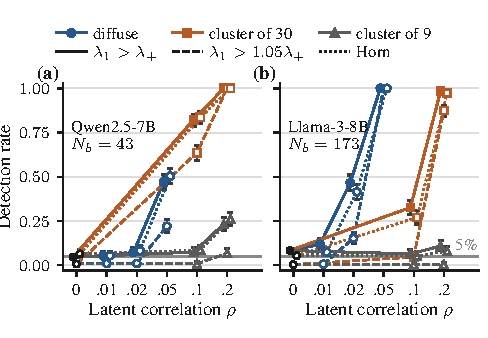
\includegraphics[width=\columnwidth]{figures/fig_power.pdf}
\caption{Detection rate (fraction of simulated matrices with a count of
at least one) against the latent correlation $\rho$ of a planted factor,
at the pass rates of (a)~Qwen2.5-7B ($N_b=43$) and (b)~Llama-3-8B
($N_b=173$) on MMLU. The $\rho$ values are placed at evenly spaced
positions, not to scale. Color: where the factor loads; black markers at
$\rho=0$: no factor. Line style: count (solid, filled markers: MP;
dashed, open: buffered; dotted, open: Horn). Whiskers: Wilson 95\%
intervals. Grey line: a detection rate of 5\%.}
\label{fig:power}
\end{figure}

Power for a diffuse factor is higher at Llama-3-8B's 173 borderline
questions, because the factor then loads four times as many questions;
power for a fixed-size cluster is lower there, because the cluster is a
smaller share of the questions (Fig.~\ref{fig:power}). At $\rho=0.05$
the MP count detects the diffuse factor in 47\% of Qwen2.5-7B
simulations and in 100\% of Llama-3-8B simulations. A 9-question cluster
at $\rho=0.2$ is detected in 23\% (MP) and 26\% (Horn) of Qwen2.5-7B
simulations and in 11\% (MP) and 8\% (Horn) of Llama-3-8B simulations.
At $\rho=0$ the false-positive rates are 4.6\% and 8.3\% (MP), 0.65\%
and 0.35\% (buffered), and 6.4\% and 5.4\% (Horn). Runs with other
numbers of borderline questions were not simulated; we expect power for a
diffuse factor to fall, and for a fixed cluster to rise, as $N_b$ shrinks.
% src: item03_power.json:models.<Qwen|Llama>.scenarios[3].power_mp_strict (0.47, 1.0); scenarios[7].{power_mp_strict 0.232/0.108, power_horn_contiguous 0.26/0.08}
% src: item03_power.json:models.<Qwen|Llama>.scenarios[0].{power_mp_strict 0.046/0.083, power_mp_buffered_1p05 0.0065/0.0035, power_horn_contiguous 0.064/0.054}

%======================================================================
\section{What the shared component couples}
\label{app:mechanism}

This appendix explains how each shared component couples the questions
of a pass, and measures what the resulting directions follow.

\paragraph{Shared noise under a shared seed.} At each generation step,
the random-number generator of a seeded request draws one exponential
random number, the noise, for every token of the vocabulary, and the
request emits the token whose probability at temperature $T$, divided by
its noise, is largest. This is Gumbel-max sampling, since the negative
logarithm of an exponential random number is a Gumbel random number:
each answer, taken alone, follows the model's distribution for its
question. Two requests with the same seed draw the same noise vector at
every step, whatever their prompts; coupled generation and
counterfactual sampling use this sharing on
purpose~\citep{corvelobenz2025coupled,ravfogel2025gumbel}. If a
shared-seed pass draws a small noise value for the token ``B'', the
sampler divides the probability of ``B'' by that small value in every
question of the pass whose letter is generated at that step, and so
favors ``B'' in all of them at once.

\begin{figure*}[t]
\centering
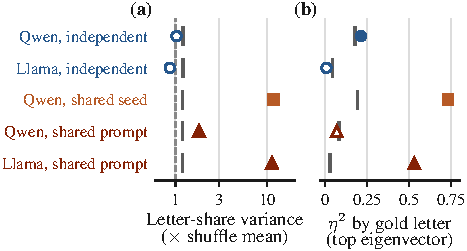
\includegraphics[width=\textwidth]{figures/fig_mechanism.pdf}
\caption{What the shared component couples, for the three
shared-component runs and the independent-draw runs of the same models.
\textbf{(a)}~Across-pass variance of a pass's share of each answer
letter, summed over the four letters and divided by its mean when each
question's answers are shuffled across passes; tick: 99th percentile
under shuffling. \textbf{(b)}~$\eta^2$ of the top eigenvector's question
loadings by gold letter; tick: 95th percentile with the gold letters
permuted. \textbf{(c)}~Correlation, over passes, between the number of a
pass's five exemplars whose answer is letter $L$ and the pass's share of
answers $L$. Filled markers: permutation $p$ below the threshold in the
legend.}
\label{fig:mechanism}
\end{figure*}

\paragraph{What the directions follow.} With a shared seed, the
across-pass variance of the fraction of a pass's answers that are each
letter, summed over letters, is 11.8 times its mean when each question's
answers are shuffled across passes (1.03 for the independent run), and
the top eigenvector's loadings separate the questions by gold letter
($\eta^2=0.73$, $p=0.0002$; Fig.~\ref{fig:mechanism}a,b). A pass whose
noise favors one letter gains on questions with that gold letter and
loses on the others, so the coupling cancels in the number correct per
pass (observed over predicted variance 0.83). Llama-3-8B with a shared
prompt copies the exemplars' letters (Fig.~\ref{fig:mechanism}c), as
few-shot prompts are known to pull answers toward their
labels~\citep{zhao2021calibrate}: per-letter $r$ between 0.35 and 0.47,
letter shares 11.3 times their shuffle mean, $\eta^2=0.53$, and an
overdispersed number correct per pass (ratio 1.51, $p=0.001$). Neither
direction groups by subject beyond chance ($p=0.23$ and $0.35$).
Qwen2.5-7B's loadings with a shared prompt do not group by gold letter
($\eta^2=0.07$, $p=0.094$), and its letter shares do not follow the
exemplars' letters (per-letter $r$ between $-0.09$ and $0.09$), but the
exemplar set matters: two passes that share an exemplar answer the
borderline questions more alike than two that share none, by 10.7 null
standard deviations when the exemplar sets are permuted across passes
(5.9 for Llama-3-8B; permutation $p=0.0005$ for both). Its loadings group
weakly by subject ($p=0.042$, uncorrected), and a same-subject exemplar
raises accuracy on borderline questions by 3.2 points ($p=0.033$); only
these two effects link the coupling to the exemplars' content. The
Qwen2.5-7B independent run shows $\eta^2=0.21$ ($p=0.023$) although its
top eigenvalue lies below its edge; we do not interpret it. The
answer-letter test of App.~\ref{app:stats} finds no pair of its
borderline questions with letters associated beyond chance, but that
test looks for single coupled pairs, not for a grouping of the loadings
by gold letter.
% src: item02_shared_randomness.json:runs.<sharedseed Qwen>.{letter_share_dispersion.ratio_obs_over_null_mean 11.8, iid_control.letter_share_dispersion.ratio_obs_over_null_mean 1.03, pass_dispersion.dispersion_ratio_obs_over_expected 0.83}
% src: item02_shared_randomness.json:runs.<sharedseed Qwen>.top_pc.loadings_eta_sq_by_subject.perm_p (0.229); runs.<sharedprompt Llama>...perm_p (0.349)
% src: item02_shared_randomness.json:runs.<sharedprompt Llama>.{exemplar_alignment.letter_echo_exemplar_count_vs_answer_share.*.r 0.35..0.47, letter_share_dispersion.ratio_obs_over_null_mean 11.3, pass_dispersion 1.51 p 0.0010, exemplar_alignment.pass_pair_similarity_shared_exemplars_borderline.z_vs_null 5.9}
% src: item02_shared_randomness.json:runs.<sharedprompt Qwen>.exemplar_alignment.{letter_echo_*.r -0.088..0.086, pass_pair_similarity_*.{z_vs_null 10.7, perm_p_upper 0.0005}, subject_match_borderline.{mean_diff 0.0324, perm_p_two_sided 0.033}}; top_pc.loadings_eta_sq_by_subject.perm_p (0.042)
% src: item02_shared_randomness.json:runs.<sharedseed Qwen>.iid_control.top_pc.loadings_eta_sq_by_gold_letter.{eta_sq 0.21, perm_p 0.023}

%======================================================================
\section{The 24-model ensemble}
\label{app:ensemble}

This appendix lists the ensemble, defines the one-ability nulls and
their validity, and gives the analyses behind Sections~\ref{sec:across}
and~\ref{sec:all4}.

\paragraph{Roster.} Five Qwen (Qwen2.5 at 0.5B, 1.5B, 3B and 7B, and
Qwen2-7B), five Mistral (Mistral-7B v0.2 and v0.3, Zephyr-7B-beta,
Ministral-8B, Mistral-Small-22B), four Llama (Llama-3.2 at 1B and 3B,
Llama-3-8B, Llama-3.1-8B), three Phi (Phi-2, Phi-3-mini, Phi-3.5-mini),
two Gemma-2 (2B and 9B), and one each of SmolLM2-1.7B, OLMo-2-7B,
Yi-1.5-6B, DeepSeek-LLM-7B and Granite-3.1-8B: ten families, five with a
single model. Phi-2 is a base model; the other 23 are instruction-tuned. Greedy accuracy in rotation 0 runs from 35.0\%
(Llama-3.2-1B) to 72.8\% (Gemma-2-9B).
% src: item07_across_model.json:observed.accuracy_per_model.{meta-llama/Llama-3.2-1B-Instruct 0.35, google/gemma-2-9b-it 0.728}

\paragraph{One-ability nulls.} Every null is simulated conditional on
every kept column staying split, so each null matrix has the observed
number of columns and the observed $\lambda_+$; each has 1000 draws. Rasch
is fitted by joint maximum likelihood. The fixed-margin null draws
uniformly among 0/1 matrices with the observed row and column sums. The
2PL treats the abilities as fixed and integrates the question parameters
over a normal population (marginal maximum likelihood); it is fitted to
all 500 columns and simulated on the split ones. The Bock--Aitkin 2PL
integrates the abilities instead, with slopes bounded by 4. The 3PL uses
the floor 0.25 for every score. The letter-aware null is a know-or-guess
model fitted to rotation 0, with each model's letter preference $\pi_m$
estimated from all four rotations. The 4-rotation letter know-or-guess
(KG-l) and uniform know-or-guess (KG-u) nulls are fitted to all four
rotations jointly, with guessing by $\pi_m$ or uniform, and simulate
every rotation.

\paragraph{Validity.} A null whose $\lambda_1$ misses the observed one
ties correctness to ability more or less tightly than the data, and its
higher eigenvalues are then not comparable with the observed ones: the
2PL, Rasch and fixed-margin nulls put the observed rotation-0 $\lambda_1$
above all their draws, and the 4-rotation know-or-guess and Bock--Aitkin
nulls put the all-4-correct $\lambda_1$ below all theirs. We therefore
use a null as evidence only if the observed $\lambda_1$ lies between its
1st and 99th percentiles, in both directions, for every score and every
null, the soft-preference null included. Under this rule the rotation-0
rank 2 is not evidence against the 2PL, and the all-4-correct verdict
rests on the 2PL and Rasch alone. The rule was set after the first
analyses, and it is necessary, not sufficient (see Size below).
% src: v3_F_softpref.json:step1_construction_family.table.full.{rot0,ge4}.{observed_pct_rank1to4_by_null, null_valid}; v3_G_familywise.json:G5_single_validity_rule.rule

\begin{table*}[t]
\caption{Construction family, soft-preference null and power. Each score
combines a model's four rotations: correct in rotation 0, in at least
$k$ of 4, or the mean. Valid nulls: those whose 1st--99th percentile
range contains the observed $\lambda_1$, each with its number of
directions beyond ability by the per-rank rule (``none'': no valid
null other than SP), for all 24 models and without Llama-3.2-1B (w/o); LA:
letter-aware; KG-l, KG-u: 4-rotation letter and uniform know-or-guess;
BA: Bock--Aitkin 2PL. Soft-preference (SP) null: rank-2 calibrated $p$;
``inv.'': the null fails the validity rule. Power: detection rate of a
planted second ability at $s=2$ by the SP null (valid, and rank 2 above
its calibrated threshold) and by the 2PL per-rank rule, 150 datasets
per $s$; --: not simulated or not valid. $^b$False-positive rate 0.69
without a second factor. $^c$From the 200 datasets of Table~\ref{tab:fw}.
The per-rank counts use 1000 draws per null; the family-wise $p_T$ of
the valid nulls (2000 new draws) are given in the text.}
\label{tab:family}
% src: v3_F_softpref.json:step1_construction_family.table.{full,no_llama1b}.<score>.{n_cols, top_eigs, ranks_beyond_ability_valid_nulls}
% src: v3_G_familywise.json:G5_single_validity_rule.sp_table_A2.{full,no_llama1b}.<score>.table_A2_cell; G5_single_validity_rule.power_sp_column.2.<score>.detect_plain_valid_and_rank2_above_cal_threshold (rot0 0.64, ge4 0.453, ge2 0.847, mean 0.193)
% src: v3_F_power.json:summary.2.by_null.2pl:ge2.detect_rank2_and_valid (0.87); summary.0.by_null.2pl:ge2.detect_rank2_and_valid (0.693); v3_G_familywise.json:G3_power.2.2pl_post.per_rank_rule_rank2_above_p99_and_valid (0.805, all-4 cell)
% src: family-wise p_T quoted in the text: v3_G_familywise.json:G1_familywise.by_score_and_null.<score>.<null>.p_T (rot0 3pl/kg_uniform4/letter_post 0.0020; ge2 2pl 0.0020, 3pl 0.8616; ge3 2pl 0.0095, rasch 0.0080, kg_letter4 0.0075, kg_uniform4 0.2769; ge4 2pl 0.0265, rasch 0.0415); v3_I_llama.json:I1_without_llama1b.table.{rot0.{3pl_post 0.0035, letter_post 0.0150}, ge4.{2pl_post 0.0595, rasch_jml 0.0890, kg_uniform4 0.1524}}.p_T
\vskip 0.05in
\centering
\begin{footnotesize}
\setlength{\tabcolsep}{2.5pt}
\begin{tabular}{@{}lcccccc@{}}
\toprule
& & & \multicolumn{2}{c}{\textbf{Valid nulls: ranks beyond ability}} & \textbf{SP: rank-2 cal.\ $p$} & \textbf{Power, $s=2$} \\
\textbf{Score} & \textbf{Cols} & $\lambda_1$--$\lambda_4$ & \textbf{24 models} & \textbf{w/o Llama-1B} & \textbf{24 / w/o} & \textbf{SP / 2PL} \\
\midrule
Rotation 0 & 460 & 85.9, 49.9, 29.7, 27.3 & 3PL 1, KG-u 1, LA 1 & 3PL, LA 0 & 0.010 / inv. & 0.64 / -- \\
$\ge1$ of 4 & 334 & 34.2, 27.2, 23.7, 21.4 & none & BA 0 & 0.750 / inv. & -- \\
$\ge2$ of 4 & 444 & 108.3, 42.3, 30.2, 23.0 & 2PL 3, 3PL 0 & 2PL 1, 3PL 0 & 0.245 / 0.280 & 0.85 / 0.87$^b$ \\
$\ge3$ of 4 & 439 & 103.4, 37.8, 25.5, 22.1 & Rasch 2, KG-l 2; 2PL, KG-u 0 & 2PL, KG-l, KG-u 0 & inv.\ / 0.285 & -- \\
All 4 & 391 & 92.1, 29.0, 23.3, 20.8 & Rasch, 2PL 0 & Rasch, 2PL, KG-u 0 & inv.\ / inv. & 0.45 / 0.81$^c$ \\
Mean & 489 & 127.5, 43.1, 28.5, 25.7 & none & none & inv.\ / inv. & 0.19 / -- \\
\bottomrule
\end{tabular}
\end{footnotesize}
\end{table*}

\paragraph{Construction family.} All-4-correct is one of several ways to
combine a model's four rotations, and a letter preference that acts on
choices the model partly knows can leak into any of them.
Table~\ref{tab:family} gives each score under the nulls valid for it.
Rotation 0 has one direction beyond ability, the letter direction of
Section~\ref{sec:across}. Without Llama-3.2-1B the per-rank rule finds
none under the valid 3PL and letter-aware nulls, but the family-wise test
rejects both ($p_T=0.0035$ and 0.015, 2000 new draws, post hoc); the
maximum is at rank 4, ranks 3 and 4 lie at the 98.5th to 99.9th
percentiles, and the letter grouping moves to eigenvector 3. Of the
rotation-combined scores, all-4-correct has none by the per-rank rule
and a marginal family-wise excess (Section~\ref{sec:all4}). On $\ge2$ of
4 the per-rank rule finds three under the 2PL (one without
Llama-3.2-1B) and none under the 3PL, and the family-wise test agrees
($p_T=0.002$ and 0.86). On $\ge3$ of 4 the per-rank rule finds two under
the Rasch and KG-l nulls and none under the 2PL and KG-u, and none
without Llama-3.2-1B; the family-wise test rejects the Rasch, KG-l and
2PL nulls ($p_T=0.008$, 0.007 and 0.009) but not KG-u (0.28). In the 2000
draws of the family-wise test the per-rank counts on $\ge3$ of 4 differ
(Rasch 1, KG-l 3, 2PL 0), a sign of how close these ranks lie to the 99th
percentiles. The SP null cannot tell whether letter preference explains
the $\ge3$ result, because it is invalid there (Family-wise test below).
On $\ge1$ of 4 only the SP null is valid, and it finds nothing
(calibrated $p$ 0.750, family-wise $p_T=0.996$); the mean has no valid
null. Removing the 23 questions
whose options refer to other options (``all of the above'', ``A and B
only'') leaves the counts of rotation 0 and all-4-correct unchanged,
lowers those of $\ge2$ (2PL 2) and $\ge3$ (Rasch 1, KG-l 0), and makes
the BA null valid on $\ge1$ of 4, with no direction.
% src: v3_G_familywise.json:G5_single_validity_rule.sp_table_A2.full.ge1.{plain_valid true, rank2_cal_p 0.75}; G1_familywise.by_score_and_null.ge1.sp_common_tau.p_T (0.9955)
% src: v3_I_llama.json:I1_without_llama1b.table.rot0.{3pl_post.{p_T 0.0035, pct_rank1to4 [96.6, 48.2, 98.5, 99.9], T_argmax_rank 4}, letter_post.{p_T 0.0150, pct_rank1to4 [88.55, 72.2, 99.2, 99.5], T_argmax_rank 4}}
% src: v3_G_familywise.json:G1_familywise.by_score_and_null.{ge2.{2pl_post.p_T 0.0020, 3pl_post.p_T 0.8616}, ge3.{rasch_jml.{p_T 0.0080, ranks_beyond_ability 1}, kg_letter4.{p_T 0.0075, ranks_beyond_ability 3}, 2pl_post.{p_T 0.0095, ranks_beyond_ability 0}, kg_uniform4.{valid true, p_T 0.2769}}}; v3_F_softpref.json:step1_construction_family.table.{full.ge3, no_llama1b.ge3}.ranks_beyond_ability_valid_nulls
% src: v3_F_softpref.json:step1_construction_family.{option_referencing (23), table.no_optref.<score>.ranks_beyond_ability_valid_nulls (ge1 {ba_a4 0}, ge2 {2pl_post 2}, ge3 {rasch_jml 1, kg_letter4 0})}

\paragraph{Soft-preference null.} In this null, model $m$ chooses option
$j$ of question $i$ in a rotation with probability proportional to
$\exp\!\big(b_{ij}+\mathbb{1}[j=g_i](a_i\theta_m+e_{mi})\big)\,\pi_m(L_j)$,
where $g_i$ is the gold option, $b_{i g_i}=0$, $L_j$ is the letter at
which the rotation shows option $j$, and $e_{mi}\sim N(0,\tau^2)$ is
shared by the four rotations of a cell and independent across models.
Ability $\theta_m$ is the only link between questions, and the letter
preference acts on every choice, also when the model partly knows the
answer. The fit is penalized maximum likelihood over the parsed choices
of all four rotations ($\tau=1.17$). Simulations keep the observed
unparseable cells, and the rotation-0 result depends on this: without
the mask the observed $\lambda_2$ lies at the 99.8th percentile of the
null, with it at the 95.1st. Refitting inflates the slopes, so we
calibrate: 200 datasets simulated from the fit, each refitted with its
own null. The calibrated $p$ of rank $j$ is the fraction of these
datasets whose $\lambda_j$ percentile is at least the observed one.
Each refitted null uses 1000 draws. Validity follows the rule above. On
rotation 0 the SP null is valid ($\lambda_1$ at the 85.7th percentile)
and rank 2 has calibrated $p=0.010$ (0.015 by the Monte Carlo
convention $(1+k)/(1+n)$, with $k$ of the $n=200$ datasets at least as
extreme), but the family-wise $p_T$ is 0.079; without Llama-3.2-1B the
null is invalid. On $\ge3$ of 4 and all-4-correct it is invalid
($\lambda_1$ at the 0th percentile), so its rejections there are not
evidence. On 200 datasets simulated from the fit, each with the null
refitted and 200 draws, the valid rotation-0 nulls reject rank 2 in 60\% (letter-aware) to 99.5\% (3PL) of datasets. The
2PL rejects rank 2 of $\ge2$ of 4 in 67.5\% of datasets at the fitted
parameters, 39\% after a bootstrap correction of the parameters' bias
and 72\% after rescaling their mean squares; the intervals cover Monte
Carlo error only, and why the bias correction lowers the rate is not
identified.
% src: v3_F_softpref.json:step2_soft_preference.fits.full__tau__sigma4.fit.tau (1.166); calibration.meta (200 datasets); SUMMARY.md F rotation-0 bullet (99.8 without mask, 95.1 with)
% src: v3_F_softpref.json:step2_soft_preference.calibration.meta.{n_datasets_per_variant 200, n_null_per_dataset 1000}; step2b_step1_nulls_under_soft_preference_truth.meta.{n_datasets 200, n_null_draws 200}; v3_G_familywise.json:G5_single_validity_rule.sp_table_A2.full.rot0.rank2_cal_p_mc (0.0149 = 3/201)
% src: v3_G_familywise.json:G5_single_validity_rule.sp_table_A2.{full.{rot0.{lambda1_pct 85.7, rank2_cal_p 0.010}, ge3.plain_valid false, ge4.plain_valid false}, no_llama1b.rot0.plain_valid false}; G1_familywise.by_score_and_null.rot0.sp_common_tau.p_T (0.07946 -> 0.079)
% src: v3_F_softpref.json:step2c_ge2_2pl_under_bias_corrected_parameters.summary.{plug_in 0.675, boot_bias_corrected 0.39, mean_square_rescaled 0.72}.frac_rank2_above_p99
% src: v3_F_softpref.json:step2b_step1_nulls_under_soft_preference_truth.summary.rot0:{letter_post 0.595, 3pl_post 0.995}.frac_rank2_above_p99

\paragraph{Predictive check.} The soft-preference model fails its
pre-set predictive check, which compares 500 datasets simulated from the
fit with the data. Per-model accuracy and letter shares fit, but the
number of rotations, 0 to 4, in which a model answers a question
correctly is covered for 82.5\% of model-by-count cells, below the
required 90\%. The weakest, letter-biased models have too many questions
correct in exactly one rotation, as expected if they choose one letter
almost deterministically, and stronger models too many correct in all
four (pooled: 0.196 observed against 0.177 simulated for one rotation,
0.382 against 0.366 for four). The calibration corrects the bias of the
fitting pipeline, not this misfit, so the soft-preference verdicts are
not fully validated.
% src: v3_F_softpref.json:step2_soft_preference.fits.full__tau__sigma4.{ppc_verdict.coverage_98.hist_model 0.825, ppc.hist_model.{observed_by_model, sim_mean_by_model}, ppc.hist_pooled.{observed[1] 0.196, sim_mean[1] 0.177, observed[4] 0.382, sim_mean[4] 0.366}}

\paragraph{Family-wise test.} The per-rank rule tests each rank at 1\%
and stops at the first rank that passes, so it can miss an excess spread
over several ranks. An audit of an earlier draft of this analysis had
raised this and had computed a
similar statistic, the largest percentile over ranks 2--4, on the same
data, and its model-pair correlations had pointed to the sibling models.
We then wrote down the family-wise test, the sibling-model test and the
single validity rule before running them, with seeds disjoint from all
earlier runs. The specification fixes the statistic, the ranks, the
decision rule and the groups; it does not make the hypothesis
independent of the data, which had suggested it. The statistic $T$ is
the largest of the percentiles of $\lambda_2$, $\lambda_3$ and
$\lambda_4$ among 2000 new null draws (ties count half); each draw's own
$T_d$ is computed against the other draws, and
$p_T=(1+\#\{d:T_d\ge T\})/2001$, at level 0.05. Table~\ref{tab:fw} gives
the results. On 200 datasets simulated from the SP fit with no second
factor (500 null draws each), the test never rejects all-4-correct under
the 2PL or Rasch; the SP model is invalid on all-4-correct, so this says
nothing about the size of the test, which the next paragraph measures.
On $\ge2$ and $\ge3$ of 4, the refitted 2PL null is valid in 98.5\%
and 100\% of the datasets, and it is valid and rejects in 98.5\% and
58\% of all datasets. The refitted Rasch null is valid in
0\% and 18\% of the datasets; it is valid and rejects in 0\% and 11\%
of all datasets, which on $\ge3$ is 61\% of the datasets in which it
is valid. The SP fit is valid on $\ge2$ but not on $\ge3$, so the
$\ge3$ rates are indicative only, and where $T=100$ the $p$ lies on a
coarse grid. Of the observed $\ge3$ rejections ($p_T$ 0.007 to 0.009,
Construction family above), the 2PL one occurs in 58\% and the Rasch
one in 11\% of datasets from a fit that the validity rule rejects on
$\ge3$, and no simulation covers the KG-l test; we draw no conclusion
from $\ge3$ of 4. In the new 2PL draws
$\lambda_4=20.83$ is above the rank-4 99th percentile (20.80), as in
replicate B, against 20.85 in the 1000 draws of Fig.~\ref{fig:spectra}d
(Monte Carlo $p=0.012$).
% src: v3_G_familywise.json:meta.{n_draws.G1 2000, n_draws.G2_datasets 200, n_draws.G2_null 500, alpha 0.05, seed_namespace}; G2_calibration_under_SP_truth.{ge4 fp_raw 0 (both), ge2.{2pl_post.fp_valid_and_p_T_lt_alpha 0.985, rasch_jml.{fp_valid_and_p_T_lt_alpha 0.0, frac_valid 0.0}}, ge3.{2pl_post.fp_valid_and_p_T_lt_alpha 0.575, rasch_jml.{fp_valid_and_p_T_lt_alpha 0.11, frac_valid 0.18}}}; G5_single_validity_rule.sp_table_A2.full.{ge2.plain_valid true, ge3.plain_valid false, ge4.plain_valid false}; Deviations 4 (grid); G1_familywise.by_score_and_null.ge4.2pl_post.rank_eigs_p99[3] (20.80)
% src: v3_G_familywise.json:G2_calibration_under_SP_truth.{ge2.2pl_post.frac_valid 0.985, ge3.2pl_post.frac_valid 1.0, ge3.rasch_jml.fp_given_valid 0.611}; no kg_letter4 key in G2 (no SP-truth family-wise simulation of KG-l)
% src: v3_C_rotations_B.json:C3_rotation_invariant.all4_correct.{spectrum.top_eigs[3] 20.82, suite.nulls.2pl_post.rank_eigs_p99[3] 20.78} (replicate B above); SUMMARY.md C(3) (MC p 0.012); prereg_G.md Motivation (audit statistic)

\paragraph{Size.} The following checks were specified after the
family-wise result and are post hoc. We simulate 300 all-4-correct
datasets from each fitted one-ability model, the 2PL and Rasch, with the
nulls' own simulator, refit both nulls to each dataset (500 draws each),
and apply the validity rule and the family-wise test
(Table~\ref{tab:fw}). The 2PL test rejects in 6.7\% of datasets under
2PL truth and 8.7\% under Rasch truth (95\% intervals 4.1--10.1\% and
5.7--12.4\%), so it is not size-controlled by the bound of 7.5\% we set
before the run. The Rasch test rejects in 6.7\% and 0.7\%, but under
Rasch truth mainly through the validity screen: the refitted Rasch null
is valid in only 23\% of those datasets. Ranking the observed $p_T$ among
the simulated ones gives calibrated values of 0.033 (2PL truth) and
0.047 (Rasch truth) for the 2PL test and 0.057 and 0.017 for the Rasch
test. The validity rule is therefore necessary, not sufficient: it does
not detect wrong slopes (the Rasch null is valid in every dataset
simulated from the 2PL fit), and it rejects the correct Rasch model,
refitted by joint maximum likelihood, in most datasets simulated from
it.
% src: v3_H_followup.json:meta.{n.H1_datasets_per_truth 300, n.H1_null_draws 500, specification (FP <= 0.075 rule)}; H1_size_under_one_ability_truth.by_truth_and_null.<truth>.<null>.{fp_valid_and_p_T_lt_alpha, fp_ci95, frac_valid (rasch/rasch 0.233; 2pl/rasch 1.0), calibrated_p_of_real}; H1_size_under_one_ability_truth.decision.{2pl_post.size_controlled false, rasch_jml.size_controlled true}

\paragraph{Sibling models.} Two models are siblings if they are versions
or fine-tunes of one base model at one parameter count, decided from
model metadata before the run: Phi-3-mini and Phi-3.5-mini;
Meta-Llama-3-8B and Llama-3.1-8B; Mistral-7B v0.2, v0.3 and
Zephyr-7B-beta; Qwen2-7B and Qwen2.5-7B. Models of one family at
different sizes are not siblings. Each of the $2\cdot2\cdot3\cdot2=24$
subsets that keep one model per group has 19 models; both nulls are
refitted to each, with 1000 draws. The 24 subsets give $p_T$ 0.09 to 0.69
and none rejects. The control removes five of the 15 models outside the
groups, chosen at random, 24 times, so that 19 models remain as well; all
24 reject ($p_T\le0.047$). The subsets of each kind overlap heavily, so
the comparison is one contrast, not 24 replicates. The random removals include
models that share a developer with the groups (Qwen2.5 at 0.5B to 3B,
Llama-3.2, Ministral-8B and Mistral-Small), and they are not matched to
the 7B--8B chat models of the groups. On all-4-correct both nulls are
valid in every sibling and random subset. In rotation 0 the 2PL and
Rasch nulls are valid in none of the 24 sibling subsets and the uniform
know-or-guess null in 17; the 3PL and letter-aware nulls are valid and
reject in all 24, so the letter direction does not depend on the
siblings.
% src: v3_G_familywise.json:meta.preregistration (G4 clusters); G4_siblings.{sibling.ge4.*.n_valid 24, random_control.ge4.*.n_valid 24, sibling.rot0.{2pl_post.n_valid 0, rasch_jml.n_valid 0, kg_uniform4.n_valid 17, 3pl_post.{n_valid 24, n_reject_raw 24}, letter_post.{n_valid 24, n_reject_raw 24}}}; meta.n_draws.G4 1000

\paragraph{Pairs and simple baselines.} The sibling result does not say
which groups matter. In a post hoc follow-up we fixed two pairs, Phi-3
and Phi-3.5-mini and Meta-Llama-3-8B and Llama-3.1-8B, and compared the
four subsets that remove one model of each pair with all 190 subsets
that remove two of the other 20 models (1000 draws per subset; every
null valid in every subset). All four pair removals lie above every
reference removal under both nulls (Table~\ref{tab:fw}); 90\% (2PL) and
74\% (Rasch) of the reference removals still reject. Removing Qwen2-7B or
Qwen2.5-7B makes the rejection stronger (mean reference $p_T$ 0.010 and
0.006 under the 2PL), so the Qwen pair is not part of the excess. The
effect is specific to the two pairs: removing the Mistral-7B v0.2 and
v0.3 near-duplicates (residual rank 3 in Table~\ref{tab:baselines})
keeps the rejection ($p_T=0.019$ under both nulls), as do the other two
removals within the Mistral group (0.004 to 0.023). Nor does removing two
strong chat models explain it: the 15 reference removals whose two models
have rotation-0 accuracy between 0.62 and 0.71 (the pair models: 0.644
to 0.684; no two other models lie inside that narrower range) give $p_T$
at most 0.052 (2PL) and 0.113 (Rasch), below every pair removal. The
letter-biased model contributes too. Without Llama-3.2-1B alone (post
hoc, 2000 new draws), $p_T$ is 0.06 (2PL) and 0.089 (Rasch), and 0.15
under the uniform know-or-guess null, which becomes valid; the secondary
statistic of the specification, $\lambda_2+\lambda_3+\lambda_4$ against
its null draws, on which no decision rests, still gives $p$ 0.023 and
0.016. Of the 19 reference removals that include Llama-3.2-1B, 12 (2PL)
and 6 (Rasch) still reject, with $p_T$ at most 0.099 and 0.130. Removing Llama-3.2-1B together with one model of
each pair gives 0.30 to 0.59 and 0.38 to 0.60 (1000 draws), close to the
pair removals alone. Table~\ref{tab:baselines} gives two simple baselines. Letter shares in
rotation 0 flag the three models whose most frequent letter exceeds half
of their replies; these shares count unparseable replies in the
denominator, whereas the preference of 0.90 for A in
Section~\ref{sec:across} is estimated over guesses. The correlations of
model pairs' residuals (observed minus 2PL-expected correctness over the
391 all-4-correct columns) rank the Phi and Llama pairs first and second
of 276. These tables find the same candidates as the spectrum; the
spectrum adds a test of whether they exceed one ability, and the
rotations attribute the larger structure to letter preference.
% src: v3_H_followup.json:meta.{P1, P2, n.H2_null_draws 1000}; H2_pair_removal_vs_reference.by_null.{2pl_post,rasch_jml}.{reference_n 190, reference_frac_valid 1.0, reference_frac_reject (0.9, 0.737), n_pairs_exceeding_p95 4, reference_mean_p_T_by_removed_model.{Qwen2-7B-Instruct 0.0098, Qwen2.5-7B-Instruct 0.0064}}
% src: v3_H_followup.json:H3_baselines.{n_models_max_share_gt_0p5 3, residual_corr.{definition, n_pairs 276, sibling_pairs}}
% src: raw_v3_H_h2.json:subsets[116] (Mistral v0.2+v0.3: 0.019/0.019), subsets[117] (v0.2+Zephyr 0.004/0.013), subsets[128] (v0.3+Zephyr 0.016/0.023)
% src: v3_I_llama.json:I2_joint_removal.from_H2_no_new_run.{accuracy_matched_rot0_accuracy.{pair_model_accuracy (0.684, 0.664, 0.644, 0.684), as_specified.summary.n 0, hostile_band.{band [0.62, 0.71], summary.{n 15, 2pl_post.p_T_min_median_max[2] 0.0519, rasch_jml.p_T_min_median_max[2] 0.1129}}}, with_llama1b.summary.{n 19, 2pl_post.{n_reject 12, max 0.0989}, rasch_jml.{n_reject 6, max 0.1299}}}
% src: v3_I_llama.json:I1_without_llama1b.table.ge4.{2pl_post.{p_T 0.0595, p_S 0.0230}, rasch_jml.{p_T 0.0890, p_S 0.01649}, kg_uniform4.{valid true, p_T 0.1524}}; I2_joint_removal.new_runs[*].{2pl_post,rasch_jml}.p_T (0.296-0.586; 0.380-0.596)

\begin{table}[t]
\caption{Simple baselines. Top: rotation-0 letter shares (unparseable
replies in the denominator) of the models whose largest share exceeds
0.5; every other model has a largest share of at most 0.35. Bottom:
correlation of model pairs' residuals after the all-4-correct 2PL fit,
with rank among 276 pairs (mean $-0.04$, standard deviation 0.08).}
\label{tab:baselines}
% src: v3_H_followup.json:H3_baselines.letter_shares_rotation0.<model>.{pi_A_B_C_D, max_share} (others max 0.348, Mistral-7B-v0.3)
% src: v3_H_followup.json:H3_baselines.residual_corr.{offdiag_mean -0.041, offdiag_sd 0.078, top10, sibling_pairs (Qwen2/Qwen2.5-7B r 0.035 rank 37)}
\vskip 0.05in
\centering
\begin{small}
\setlength{\tabcolsep}{4pt}
\begin{tabular}{@{}lcccc@{}}
\toprule
\textbf{Model} & A & B & C & D \\
\midrule
Llama-3.2-1B & 0.81 & 0.04 & 0.09 & 0.05 \\
Qwen2.5-0.5B & 0.23 & 0.06 & 0.12 & 0.58 \\
SmolLM2-1.7B & 0.07 & 0.20 & 0.17 & 0.56 \\
\midrule
\textbf{Model pair} & & & $r$ & \textbf{Rank} \\
\midrule
Phi-3-mini, Phi-3.5-mini & & & 0.40 & 1 \\
Meta-Llama-3-8B, Llama-3.1-8B & & & 0.27 & 2 \\
Mistral-7B v0.2, v0.3 & & & 0.20 & 3 \\
Mistral-7B v0.3, Meta-Llama-3-8B & & & 0.19 & 4 \\
Mistral-7B v0.2, Zephyr-7B & & & 0.17 & 5 \\
Qwen2-7B, Qwen2.5-7B & & & 0.03 & 37 \\
\bottomrule
\end{tabular}
\end{small}
\end{table}

\begin{table}[t]
\caption{Family-wise test on all-4-correct (2PL and Rasch nulls; reject
at $p_T<0.05$). Sibling and random subsets: subsets that reject, and
the range or maximum of $p_T$. Pairs: the four removals of one Phi and
one Llama model, and the 190 removals of two other models (fraction that
reject, maximum $p_T$). Unparseable: replies imputed, the 95 questions
whose score they affect dropped, or all 217 questions with any dropped
(1000 draws each).
Size: rejection rate in 300 datasets simulated from each fitted
one-ability model, and the observed $p_T$ calibrated against them (2PL
truth, Rasch truth).
Power: family-wise / per-rank rule, 200 datasets per slope $s$.}
\label{tab:fw}
% src: v3_G_familywise.json:G1_familywise.by_score_and_null.ge4.{2pl_post,rasch_jml}.{pct_rank1to4, p_T}; G4_siblings.{sibling,random_control}.ge4.*.{n_reject_raw, p_T_min_median_max}; G6_unparsed_variants.{ge4__impute,ge4__drop_affected,ge4__drop_any}.nulls.*.p_T; G3_power.{1,2}.*.{detect_G1_raw, per_rank_rule_rank2_above_p99_and_valid}
% src: v3_H_followup.json:H2_pair_removal_vs_reference.by_null.*.{pair_removals[*].p_T, reference_frac_reject, reference_max}; H1_size_under_one_ability_truth.by_truth_and_null.<truth>.<null>.{fp_valid_and_p_T_lt_alpha, calibrated_p_of_real}
\vskip 0.05in
\centering
\begin{small}
\setlength{\tabcolsep}{4pt}
\begin{tabular}{@{}lcc@{}}
\toprule
& \textbf{2PL} & \textbf{Rasch} \\
\midrule
Pct.\ of $\lambda_2,\lambda_3,\lambda_4$ & 71.8, 98.5, 99.1 & 94.6, 97.0, 98.6 \\
$p_T$, 24 models & 0.026 & 0.041 \\
Sibling subsets & 0/24 (0.09--0.65) & 0/24 (0.12--0.69) \\
Random subsets & 24/24 ($\le$0.047) & 24/24 ($\le$0.046) \\
Pair removals & 0/4 (0.22--0.69) & 0/4 (0.32--0.38) \\
Other two removed & 0.90 ($\le$0.099) & 0.74 ($\le$0.133) \\
Unparseable: impute & 0.019 & 0.042 \\
\quad drop 95 & 0.036 & 0.043 \\
\quad drop 217 & 0.23 & 0.12 \\
Size, 2PL truth & 0.067 & 0.067 \\
Size, Rasch truth & 0.087 & 0.007 \\
Calibrated $p_T$ & 0.033, 0.047 & 0.057, 0.017 \\
Power, $s=1$ & 0.34 / 0.06 & 0.21 / 0.08 \\
Power, $s=2$ & 0.92 / 0.81 & 0.87 / 0.80 \\
\bottomrule
\end{tabular}
\end{small}
\end{table}

\paragraph{Power.} To measure what the all-4-correct verdict can
exclude, we add a second ability $\theta_{2,m}\sim N(0,1)$, independent
of $\theta_m$, with slope $s$ to the gold-option term
$a_i\theta_m+e_{mi}$ of the 180 STEM questions, simulate datasets from
the soft-preference fit, and refit every null. The fit's median slope
$|a_i|$ is 1.08, so $s=1$ is about a typical first-ability slope; at
$s=2$ the planted term carries on average 60\% of the variance across
models of a STEM question's gold-option term (30\% at $s=1$).
Table~\ref{tab:fw} gives the all-4-correct power from 200 datasets per
$s$. The datasets come from the soft-preference fit, which is invalid on
all-4-correct ($\lambda_1$ below all its draws), so these rates are
indicative, not a measurement for data like ours. An
earlier simulation with 150 datasets per $s$ gives the power
column of Table~\ref{tab:family}; in it the 2PL per-rank rule never
fires on all-4-correct without a planted factor, but fires in 69\% of
$\ge2$ datasets. The SP rule fires in at most 2\% of datasets at $s=0$.
% src: raw_v3_F_sp_fits.npz:full__tau__sigma4__a (median |a| 1.076); v3_F_power.json:meta.{n_datasets_per_s 150, block}; summary.{2,1}.planted_var_share_stem_mean (0.595, 0.299); summary.0.by_null.{2pl:ge4 0.000, 2pl:ge2 0.693}; v3_G_familywise.json:meta.n_draws.G3_datasets_per_s (200)
% src: v3_G_familywise.json:G5_single_validity_rule.power_sp_column.0.<score>.detect_plain_valid_and_rank2_above_cal_threshold (max 0.02)

\paragraph{Letter preference.} Figure~\ref{fig:letters} shows the
evidence of Section~\ref{sec:across}. The original-option correlation in
panel~(b) follows from the shown-letter correlation and the cyclic shape
of the letter profile, so it adds no separate evidence; the same-question
correlation does. Eigenvector 1 also carries a letter part ($\eta^2=0.22$
by gold letter), and eigenvectors 3 and 4 group only slightly
($\eta^2=0.087$ and $0.061$). The same models carry eigenvector 2 in
every rotation: their scores correlate with those of rotation 0 at
$|r|=0.95$ to 0.98. Without Llama-3.2-1B, refitted on 23 models, no rank
from 2 upward exceeds the 3PL or letter-aware 99th percentile except
rank 4, by 0.35 and 0.57; the family-wise test rejects both nulls
(Construction family above), and the letter grouping moves to
eigenvector 3 ($\eta^2=0.21$ by gold letter). In expectation,
benchmark-level scores cannot carry a letter preference when gold letters
are balanced, as nearly here (118, 124, 129, 129 for A to D).
% src: results/mmlu_ensemble_rotations.npz:gold_idx (bincount 118, 124, 129, 129)
% src: v3_B_extra.json:letter_analysis.eigenvectors[0,2,3].eta_sq_by_shown_gold_letter.eta_sq (0.22, 0.087, 0.061); v3_C1b_letter_following.json:A.eigvec2.{1,2,3}.model_score_match_abs_r (0.98/0.96/0.95)
% src: v3_B_leave_one_out.json:without_llama_3_2_1b.rot0_suite.nulls.{3pl_post,letter_post}.observed_ranks_above_p99 ([4]); v3_summary_derived.json:loo23_rot0_rank4_obs_minus_p99 (0.35, 0.57)

\begin{figure}[tb]
\centering
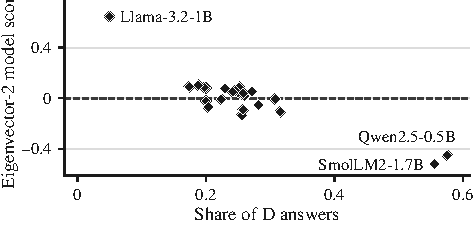
\includegraphics[width=\columnwidth]{figures/fig_letters.pdf}
\caption{Eigenvector 2 of the 24-model matrix is answer-letter
preference. \textbf{(a)}~Each model's score on eigenvector 2 in rotation
0 against its fraction of answers that are D ($r=-0.90$, permutation
$p=10^{-4}$); filled: the three models at the ends. \textbf{(b)}~For
rotations 1--3, correlation of each question's loading on eigenvector 2
with the rotation-0 mean loading of a gold letter, taken at the letter
now shown (shown letter) or at the original letter (original letter),
and with the question's own rotation-0 loading (same question); 440, 433
and 448 questions.}
\label{fig:letters}
% src: v3_B_extra.json:letter_analysis.eigenvectors[1].model_score_corr.share_D.{r -0.90, perm_p_two_sided 1.0e-04}; v3_C1b_letter_following.json:A.eigvec2.{1,2,3}.{r_shown, r_orig, r_direct, n_questions 440/433/448}
\end{figure}

\paragraph{The remaining eigenvectors.} The all-4-correct eigenvector 2
groups its question loadings by subject ($\eta^2=0.21$, $p=0.001$), but
a cubic in question difficulty explains 39\% of its loading variance,
and after removing it the grouping is at chance ($p=0.24$). Of the
borderline directions of the other scores, only $\ge2$ ranks 2 and 3
group by subject after this removal ($p=0.010$ and $0.034$, uncorrected
over eight eigenvectors). The models' scores on the all-4-correct
eigenvector 4, below $\lambda_+$, group by family ($\eta^2=0.74$,
$p=0.006$); in rotation 0, after a Holm correction, only eigenvector 4
aligns with family ($p=0.017$), and same-family model pairs correlate
little more than other pairs (mean $r$ 0.414 against 0.375, $p=0.085$
by a permutation of model labels).
% src: v3_C_rotations_A.json:C3_rotation_invariant.all4_correct.letters_subject_family.eigenvectors[1].eta_sq_by_subject.{eta_sq 0.207, perm_p 0.001}
% src: v3_F_softpref.json:step4_characterization.targets.full__ge4.2.{r2_loading_on_cubic_difficulty 0.386, eta_sq_subject_after_cubic.perm_p 0.242}; targets.full__ge2.{2,3}.eta_sq_subject_after_cubic.perm_p (0.010, 0.034)
% src: v3_C_rotations_A.json:C3_rotation_invariant.all4_correct.letters_subject_family.eigenvectors[3].eta_sq_model_scores_by_family.{eta_sq 0.74, perm_p 0.006}
% src: item10_pair_correlations.json:family_tests_holm.eigvec4_family_eta_sq (0.017); qap_model_label_permutation.{mean_r_same 0.414, mean_r_cross 0.375, perm_p_one_sided 0.085}

\paragraph{Replicates and near ties.} Replicate B differs from A in the
chosen option in 6 of 48{,}000 cells, so it tests GPU nondeterminism,
not resampling; the largest eigenvalue difference between the replicates
over every matrix compared is 0.081. A near tie is a cell whose two most
probable first-token letters differ by less than 0.13 nats in log
probability, in either replicate (5.0\% of cells). Setting near ties to
the majority answer over rotations leaves every verdict unchanged.
Dropping the 297 questions with a rotation-0 near tie leaves 203, with
less power; rank 2 then falls below the letter-aware 99th percentile but
stays above the 3PL's. Both nulls are valid for this variant (observed
$\lambda_1$ near their 13th and 14th percentiles).
% src: v3_F_softpref.json:step4_characterization.meta.replicate_B_difference.{n_cells_choice_differs 6, n_cells 48000}; v3_C4_replicate_agreement.json:max_abs_eig_diff_overall (0.081)
% src: v3_C5_near_ties.json:{frac_near_tie_cells 0.050, n_questions_with_a_rot0_near_tie 297, refitted_variants.*.suite.*}; refitted_variants.rot0_drop_questions_with_rot0_near_tie.suite.nulls.{3pl_post,letter_post}.mc_pvalue_per_rank[0] (0.870, 0.861: lambda_1 at about the 13th and 14th pct)

\end{document}
